\subsection*{Задача 2.1}

\underline{Условие:} имеется участок с N станками. Среднее время между наладками составляет Tc минут, среднее время наладки – Ts минут. Все потоки случайных событий считать пуассоновскими. Построить график зависимости числа простаивающих станков от числа наладчиков. Построить график зависимости числа станков, ожидающих обслуживания, от числа наладчиков. Построить график зависимости среднего числа занятых наладчиков от их числа. Построить график зависимости коэффициента занятости наладчиков от их числа.\par

\underline{Решение:}\par

Для расчета вероятности, при которой все станки будут налажены, можно воспользоваться формулой:

\begin{equation}
    P_{0}=\frac{1}{1+ \sum _{i=1}^{M}\frac{ \prod_{j=1}^{i} \left( N-j+1 \right)  \cdot  \lambda ^{i}}{i! \cdot  \mu ^{i}}+ \sum _{k=M+1}^{N}\frac{ \prod_{j=1}^{k} \left( N-j+1 \right) }{M! \cdot M^{k-M}} \cdot  \left( \frac{ \lambda }{ \mu } \right) ^{k}}
\end{equation} 

где  \( P_{0}-  \) вероятность, при которой все станки будут налажены;\par

 \( M-  \) количество наладчиков;\par

 \( N-  \) количество станков;\par

 \(  \lambda -  \) интенсивность поломки станков;\par

 \(  \mu -  \) интенсивность наладки станков.\par

Для расчета числа ожидающих наладки станков можно воспользоваться формулой 19:\par

\begin{equation} 
    \overline{N}_{ожид.}=P_{0} \cdot  \sum _{k=M+1,~ i=1}^{N, N-M}\frac{i \cdot  \prod_{j=1}^{k} \left( N-j+1 \right) }{M! \cdot M^{k-M}} \cdot  \left( \frac{ \lambda }{ \mu } \right) ^{k} 
\end{equation} \par

где  \( \overline{N}_{ожид.}-  \) среднее количество ожидающих наладки станков.\par

Для расчета числа простаивающих станков можно воспользоваться формулой 20:\par

\begin{equation}
    \overline{N}_{прост.}=P_{0} \cdot  \sum _{i=1}^{M}\frac{i \cdot  \prod_{j=1}^{i} \left( N-j+1 \right)  \cdot  \lambda ^{i}}{i! \cdot  \mu ^{i}} + P_{0} \cdot  \sum _{k=M+1}^{N}\frac{k \cdot  \prod_{j=1}^{k} \left( N-j+1 \right) }{M! \cdot M^{k-M}} \cdot  \left( \frac{ \lambda }{ \mu } \right) ^{k}
\end{equation} \par

где  \( \overline{N}_{прост.}-  \) среднее количество простаивающих станков.\par

Для расчета среднего числа занятых наладчиков можно воспользоваться формулой 21:\par

\begin{equation}
    \overline{M}_{зан.}=P_{0} \cdot  \sum _{i=1}^{M}\frac{i \cdot  \prod_{j=1}^{i} \left( N-j+1 \right)  \cdot  \lambda ^{i}}{i! \cdot  \mu ^{i}} + P_{0} \cdot M \cdot  \sum _{k=M+1}^{N}\frac{ \prod_{j=1}^{k} \left( N-j+1 \right) }{M! \cdot M^{k-M}} \cdot  \left( \frac{ \lambda }{ \mu } \right) ^{k}
\end{equation} \par

где  \( \overline{M}_{зан.}-  \) среднее количество занятых наладчиков.\par

Для расчета коэффициента занятости наладчиков от их числа можно воспользоваться формулой 22:\par

 \begin{equation}
    k_{M}=\frac{\overline{M}_{зан.}}{M} 
\end{equation} \par

 \( k_{M}-  \) коэффициент занятости наладчиков.\par


\begin{figure}[H]
	\begin{center}
        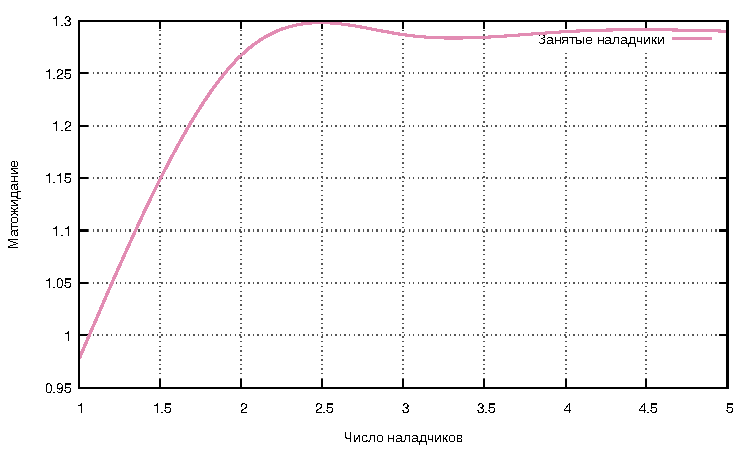
\includegraphics{/z2/mz.pdf}
        \caption{Зависимость математического ожидания ожидающих наладки станков от количества наладчиков}
	\end{center}
\end{figure}

\begin{figure}[H]
	\begin{center}
        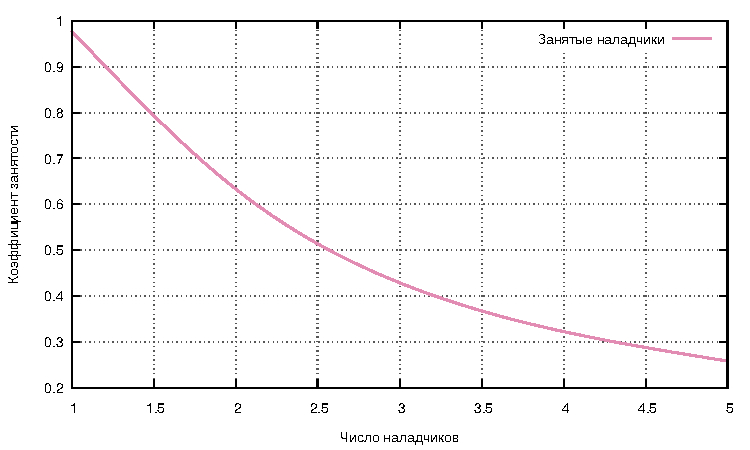
\includegraphics{/z2/mzdn.pdf}
        \caption{Зависимость математического ожидания простаивающих станков от количества наладчиков}
	\end{center}
\end{figure}

\begin{figure}[H]
	\begin{center}
        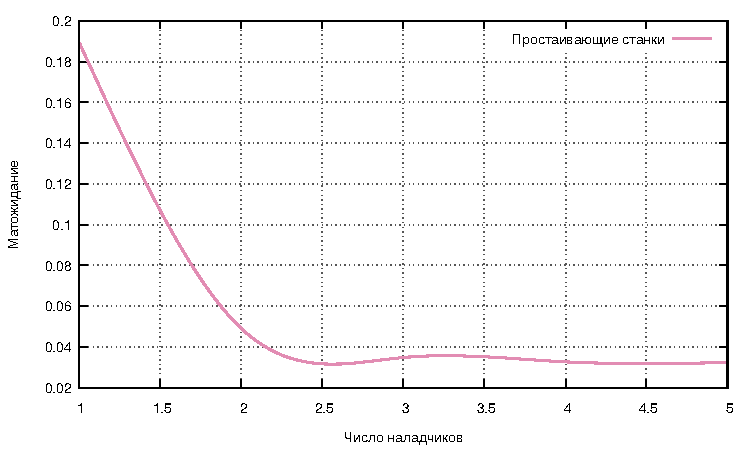
\includegraphics{/z2/nprost.pdf}
        \caption{Зависимость математического ожидания простаивающих станков от количества наладчиков}
	\end{center}
\end{figure}

\begin{figure}[H]
	\begin{center}
        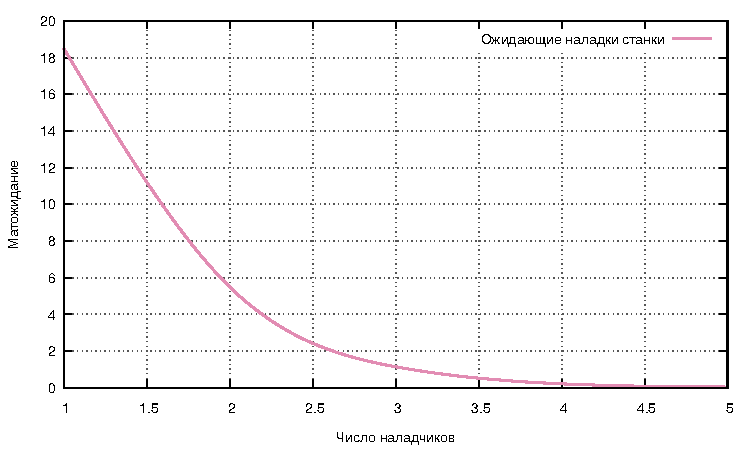
\includegraphics{/z2/nozh.pdf}
        \caption{Зависимость коэффициента занятости наладчиков от их числа}
	\end{center}
\end{figure}